\documentclass[12pt,journal,compsoc]{IEEEtran}

\usepackage{array}
\usepackage{bytefield}
\usepackage{graphicx}
\usepackage{listings}
\usepackage{slashbox}
\usepackage{tikz}

\lstset{
  frame=tb,
  language=C,
  aboveskip=3mm,
  belowskip=3mm,
  showstringspaces=false,
  columns=flexible,
  basicstyle={\small\ttfamily},
  numbers=none,
  breaklines=true,
  breakatwhitespace=true,
  tabsize=3
}

\hyphenation{op-tical net-works semi-conduc-tor}

\newcounter{mcount}
\setcounter{mcount}{0}

\begin{document}

\title{Reliable Multicast tool using UDP/IP}

\author{David Gong, Stephen Hamilton}% <-this % stops a space
\date{Sunday, September 21, 2014}

\IEEEtitleabstractindextext{%
\begin{abstract}
Our goal is to develop a multicast system capable of sending packets in agreed order utilizing the UDP/IP protocol.  In order to accomplish this task, we will implement a ring protocol where a token is passed in order to establish the control of sending packets.  A node will only be able to send packets when the node is in possession of the token.  
\end{abstract}
}
\maketitle

\section{Introduction}

\IEEEPARstart{T}{his} multicast ring protocol works by utilizing a token to control the flow of packets multicasted to all processes.  The general idea is that once the processes are initiated, the first process (machine\_id = 1) will generate the first token.  If that machine has data to send, it will send data up to the maximum flow control value (pre defined).  Once it has sent the data, it will send the token to the group with the process id set to the next receiving process.  The next process then checks the min(token.aru, previous token.aru) and writes all the data it has up to that aru from the data structure to the file. It looks at the rtr and resends any packets that it has. Finally, it sends the packets it needs to send, updates the token sequence number, rtr, and sends the token to the next process. So the cycle repeats.

\section{Design}

\subsection{Assumptions}
Before delving into the specifics of our protocol, there are a few assumptions on which the success of our protocol depends.
\begin{itemize}
\item Machine ids will be in sequential and continuous order up to the maximum number of machines (10).
\end{itemize}
With these assumptions, we can describe a successful multicast protocol for agreed data ordering over UDP.

\subsection{Token Design}


\begin{lstlisting}
// Structure of token.
int sequence;//Sequence of last message
int aru;//Sequence of all rcv up to
int fcc;//Flow control/Max send size
int rtr[fcc];//Array of Retransmit requests
int rcv_process_id;//Receiving process id
\end{lstlisting}

\subsection{Data Structure}
The data structure we plan to implement is a linked list.  This list will contain all the sent packets that are greater than min(token.aru, previous token.aru).  It will be implemented in a struct as follows:
\begin{lstlisting}
struct packet_structure {
	int token_sequence;
	int received;
	int machine_index;
	int packet_index;
	int random_number;
	char data[packet_size];
	struct packet_structure *next;
	}
\end{lstlisting}

The packet structure contains the overall token sequence, whether or not the packet was received, the machine\_index of the sender, the packet\_index of the sender's sequence, the random number, the 1200 additional payload bytes, along with the pointer to the next packet.\\
\\
As data is received, it is put into the linked list of packets.  If a packet is received out of sequence, then a placeholder packet is created with received set to 0.  Then the packet further in the sequence is populated with the received data.  Once the token is received, the packets that are at sequence number min(token.aru, prevtoken.aru) or before are written to the log and deallocated.  This allows each process to maintain all the packets that are not verified as as received by all processes in memory.  Since they are in memory, they can be re-sent if they appear in the token retransmission request (rtr).\\
\\
We also plan to utilize the following variables.\\
\begin{verbatim}
struct initializers {
	struct packet_structure *head;
	struct packet_structure *tail;
	FILE *logfile;
	int packets_to_send;
	int machine_index;
	int packet_index = 0;
	int total_machines;
	int loss_rate;
	int token_timeout;
	int prior_token_aru = 0;
	}
\end{verbatim}

\subsection{State Machine}

\begin{center}
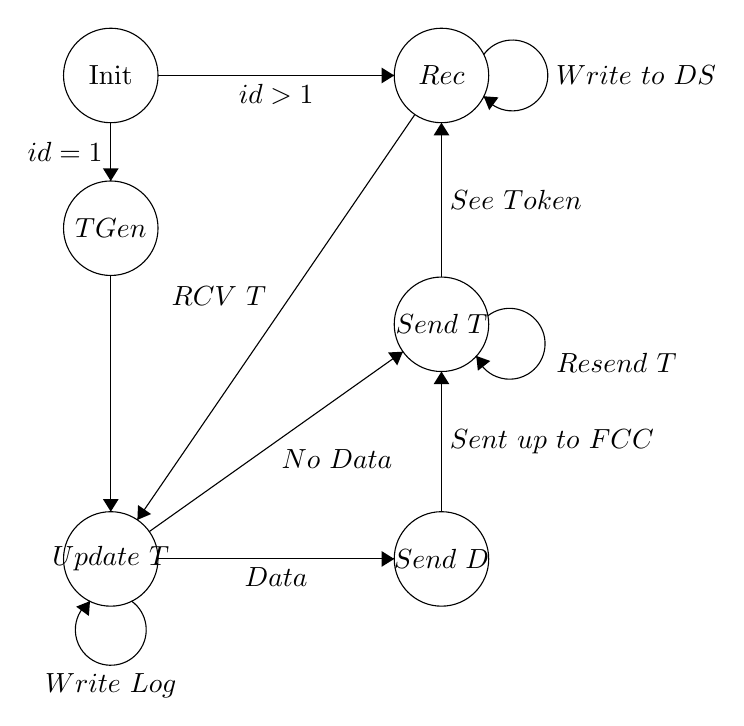
\begin{tikzpicture}[scale=0.2]
\tikzstyle{every node}+=[inner sep=0pt]
\draw [black] (4.7,-3.1) circle (3);
\draw (4.7,-3.1) node {$\mathrm{Init}$};
\draw [black] (4.7,-12.8) circle (3);
\draw (4.7,-12.8) node {$TGen$};
\draw [black] (25.7,-3.1) circle (3);
\draw (25.7,-3.1) node {$Rec$};
\draw [black] (4.7,-33.8) circle (3);
\draw (4.7,-33.8) node {$Update\mbox{ }T$};
\draw [black] (25.7,-33.8) circle (3);
\draw (25.7,-33.8) node {$Send\mbox{ }D$};
\draw [black] (25.7,-18.9) circle (3);
\draw (25.7,-18.9) node {$Send\mbox{ }T$};
\draw [black] (4.7,-6.1) -- (4.7,-9.8);
\fill [black] (4.7,-9.8) -- (5.2,-9) -- (4.2,-9);
\draw (4.2,-7.95) node [left] {$id=1$};
\draw [black] (7.7,-3.1) -- (22.7,-3.1);
\fill [black] (22.7,-3.1) -- (21.9,-2.6) -- (21.9,-3.6);
\draw (15.2,-3.6) node [below] {$id>1$};
\draw [black] (28.38,-1.777) arc (144:-144:2.25);
\draw (32.95,-3.1) node [right] {$Write\mbox{ }to\mbox{ }DS$};
\fill [black] (28.38,-4.42) -- (28.73,-5.3) -- (29.32,-4.49);
\draw [black] (6.023,-36.48) arc (54:-234:2.25);
\draw (4.7,-41.05) node [below] {$Write\mbox{ }Log$};
\fill [black] (3.38,-36.48) -- (2.5,-36.83) -- (3.31,-37.42);
\draw [black] (7.7,-33.8) -- (22.7,-33.8);
\fill [black] (22.7,-33.8) -- (21.9,-33.3) -- (21.9,-34.3);
\draw (15.2,-34.3) node [below] {$Data$};
\draw [black] (7.15,-32.06) -- (23.25,-20.64);
\fill [black] (23.25,-20.64) -- (22.31,-20.69) -- (22.89,-21.51);
\draw (19.06,-26.85) node [below] {$No\mbox{ }Data$};
\draw [black] (28.64,-18.365) arc (128.0546:-159.9454:2.25);
\draw (32.96,-21.32) node [right] {$Resend\mbox{ }T$};
\fill [black] (27.91,-20.91) -- (28.01,-21.85) -- (28.8,-21.23);
\draw [black] (25.7,-15.9) -- (25.7,-6.1);
\fill [black] (25.7,-6.1) -- (25.2,-6.9) -- (26.2,-6.9);
\draw (26.2,-11) node [right] {$See\mbox{ }Token$};
\draw [black] (24.01,-5.58) -- (6.39,-31.32);
\fill [black] (6.39,-31.32) -- (7.26,-30.95) -- (6.43,-30.38);
\draw (14.6,-17.1) node [left] {$RCV\mbox{ }T$};
\draw [black] (4.7,-15.8) -- (4.7,-30.8);
\fill [black] (4.7,-30.8) -- (5.2,-30) -- (4.2,-30);
\draw [black] (25.7,-30.8) -- (25.7,-21.9);
\fill [black] (25.7,-21.9) -- (25.2,-22.7) -- (26.2,-22.7);
\draw (26.2,-26.35) node [right] {$Sent\mbox{ }up\mbox{ }to\mbox{ }FCC$};
\end{tikzpicture}
\end{center}

\subsection{Functions}
In this design, we plan to utilize many functions in order to carry out the described algorithm.  \\
\begin{verbatim}
function init()
   Waits for start_mcast to singal start
   
function token_generate()
  returns token;
  generates the first token

function update_token
		(struct token *t, int sequence) 
  updates the token with sequence number
  
function write_log
		(struct initializers *i)
  writes to log for all received data
  
function update_rtr
		(struct initializers *i)
  Writes rtr to token based on missing 
  	packets
  
function send_data
		(struct initializers *i, struct token *t)
   returns new sequence number
   
function send_token
		(struct token *t)
   sends the current token to the next 
   	process
   
function add_packet
		(initializers *i, 
		struct packet_structure *p)
   adds an incoming packet to the data 
   	structure.	

function send_rtr_packets
		(initializers *i, struct token *t)
   sends packets needed to be 
   	retransmitted from token rtr
 
\end{verbatim}


\section{Results}
TBD

\section{Conclusion}
TBD

\section{Discussion}
TBD


\end{document}


